\documentclass[border=0.8ex,svgnames,tikz,varwidth]{standalone}
\usepackage{amsmath,mathtools}
\usepackage{fontspec}
\setmainfont{Source Serif 4}
\setsansfont{Source Sans 3}
\setmonofont{Source Code Pro}
\usetikzlibrary{positioning,calc,fit,shapes,arrows.meta}
\begin{document}
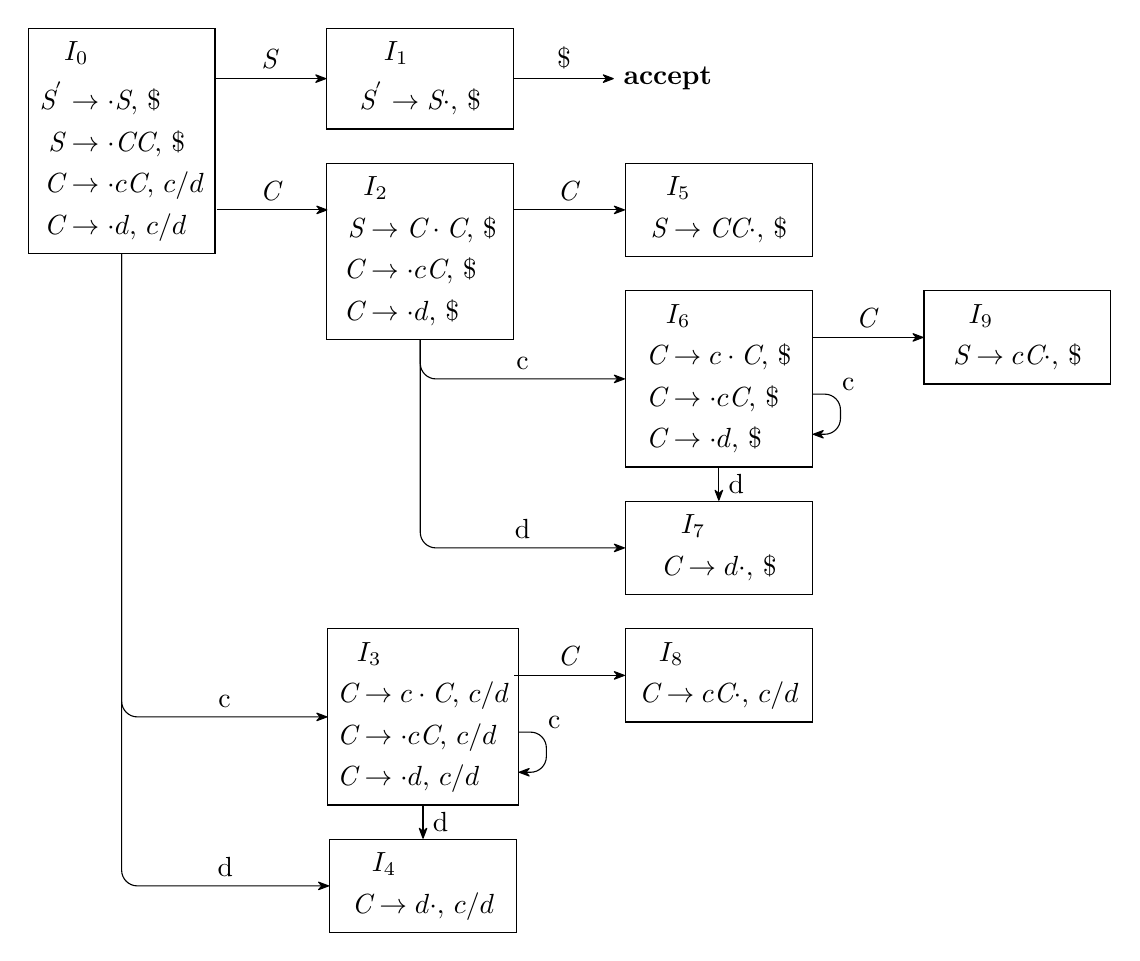
\begin{tikzpicture}
  \begin{scope}[
    every node/.style={
      rectangle,
      draw,
      minimum width=6.75em,
    },
    setanchor/.style={
      anchor=north west,
    },
    ]
    % I0
    \node (I0) at (0,0)
    {$\begin{aligned}
      & I_{0}\\
      \textit{S}^{'} &\rightarrow \cdot\textit{S},\,\$\\
      \textit{S} &\rightarrow \cdot\textit{C}\textit{C},\,\$\\
      \textit{C} &\rightarrow \cdot{}c\textit{C},\,c/d\\
      \textit{C} &\rightarrow \cdot{}d,\,c/d
    \end{aligned}$};

    % I1
    \node [right=4em of I0.north east,setanchor] (I1)
    {$\begin{aligned}
      & I_{1}\\
      \textit{S}^{'} &\rightarrow \textit{S}\cdot,\,\$
    \end{aligned}$};

    % I2
    \node [below=1.2em of I1] (I2)
    {$\begin{aligned}
      & I_{2}\\
      \textit{S} &\rightarrow \textit{C}\cdot\textit{C},\,\$\\
      \textit{C} &\rightarrow \cdot{}c\textit{C},\,\$\\
      \textit{C} &\rightarrow \cdot{}d,\,\$
    \end{aligned}$};

    % I5
    \node [right=4em of I2.north east,setanchor] (I5)
    {$\begin{aligned}
      & I_{5}\\
      \textit{S} &\rightarrow \textit{C}\textit{C}\cdot,\,\$
    \end{aligned}$};

    % I6
    \node [below=1.2em of I5] (I6)
    {$\begin{aligned}
      & I_{6}\\
      \textit{C} &\rightarrow c\cdot\textit{C},\,\$\\
      \textit{C} &\rightarrow \cdot{}c\textit{C},\,\$\\
      \textit{C} &\rightarrow \cdot{}d,\,\$
    \end{aligned}$};

    % I9
    \node [right=4em of I6.north east,setanchor] (I9)
    {$\begin{aligned}
      & I_{9}\\
      \textit{S} &\rightarrow c\textit{C}\cdot,\,\$
    \end{aligned}$};

    % I7
    \node [below=1.2em of I6] (I7)
    {$\begin{aligned}
      & I_{7}\\
      \textit{C} &\rightarrow d\cdot,\,\$
    \end{aligned}$};

    % I8
    \node [below=1.2em of I7] (I8)
    {$\begin{aligned}
      & I_{8}\\
      \textit{C} &\rightarrow c\textit{C}\cdot,\,c/d
    \end{aligned}$};

    % I3
    \node [left=10.75em of I8.north west,setanchor] (I3)
    {$\begin{aligned}
      & I_{3}\\
      \textit{C} &\rightarrow c\cdot\textit{C},\,c/d\\
      \textit{C} &\rightarrow \cdot{}c\textit{C},\,c/d\\
      \textit{C} &\rightarrow \cdot{}d,\,c/d
    \end{aligned}$};

    % I4
    \node [below=1.2em of I3] (I4)
    {$\begin{aligned}
      & I_{4}\\
      \textit{C} &\rightarrow d\cdot,\,c/d
    \end{aligned}$};
  \end{scope}
  \begin{scope}[
    myarrow/.style={
      ->,
      rounded corners=2mm,
      >=Stealth[round],
      % very thick,
    },
    ]
    % Path I0
    \draw [myarrow] (I1.west) ++(-4em,0) -- node [above] {\textit{S}} ++(4em,0);
    \draw [myarrow] (I5.west) ++(-14.75em,0) -- node [above] {\textit{C}} ++(4em,0);
    \draw [myarrow] (I0) |- (I3);
    \draw [myarrow] (I0) |- (I4);
    \node [above] at ($(I0.south |- I3.west)!0.5!(I3.west)$) {c};
    \node [above] at ($(I0.south |- I4.west)!0.5!(I4.west)$) {d};

    % Path I1
    \draw [myarrow] (I1.east) -- node [above] {\(\$\)} ++(3.6em,0) node [right] {\textbf{accept}};

    % Path I2
    \draw [myarrow] (I5.west) ++(-4em,0) -- node [above] {\textit{C}} ++(4em,0);
    \draw [myarrow] (I2) |- (I6);
    \draw [myarrow] (I2) |- (I7);
    \node [above] at ($(I2.south |- I6.west)!0.5!(I6.west)$) {c};
    \node [above] at ($(I2.south |- I7.west)!0.5!(I7.west)$) {d};

    % Path I3
    \draw (I3.east) ++ (0,-0.55em) coordinate (oI3iI3start);
    \draw (I3.east) ++ (0,-2em) coordinate (oI3iI3end);
    \draw [myarrow] (oI3iI3start) -- ++(1em,0) |- (oI3iI3end);
    \draw [myarrow] (I3) -- node [right] {d} (I4);
    \draw [myarrow] (I8.west) ++(-4em,0) -- node [above] {\textit{C}} ++(4em,0);
    \node [label=right:c,below left=-1em] at (oI3iI3start) {};

    % Path I6
    \draw (I6.east) ++ (0,-0.55em) coordinate (oI6iI6start);
    \draw (I6.east) ++ (0,-2em) coordinate (oI6iI6end);
    \draw [myarrow] (oI6iI6start) -- ++(1em,0) |- (oI6iI6end);
    \draw [myarrow] (I6) -- node [right] {d} (I7);
    \draw [myarrow] (I9.west) ++(-4em,0) -- node [above] {\textit{C}} ++(4em,0);
    \node [label=right:c,below left=-1em] at (oI6iI6start) {};
  \end{scope}
\end{tikzpicture}
\end{document}
